\documentclass{sig-alternate}
  \pdfpagewidth=8.5truein
  \pdfpageheight=11truein

%\clubpenalty=10000
%\widowpenalty = 10000

%%\documentclass{sig-alternate-2014}
%\newfont{\mycrnotice}{ptmr8t at 7pt}
%\newfont{\myconfname}{ptmri8t at 7pt}
%\let\crnotice\mycrnotice%
%\let\confname\myconfname%


%\permission{Permission to make digital or hard copies of all or part of this work for personal or classroom use is granted without fee provided that copies are not made or distributed for profit or commercial advantage and that copies bear this notice and the full citation on the first page. Copyrights for components of this work owned by others than ACM must be honored. Abstracting with credit is permitted. To copy otherwise, or republish, to post on servers or to redistribute to lists, requires prior specific permission and/or a fee. Request permissions from permissions@acm.org.}

% --- Author Metadata here ---
\conferenceinfo{SAC'16,}{April 4-8, 2016, Pisa, Italy.}
\CopyrightYear{2016} % Allows default copyright year (2002) to be over-ridden - IF NEED BE.
\crdata{978-1-4503-3739-7/16/04...\$15.00.\\
http://dx.doi.org/xx.xxxx/xxxxxxx.xxxxxxx
}  % Allows default copyright data (X-XXXXX-XX-X/XX/XX) to be over-ridden.
% --- End of Author Metadata ---


\usepackage{cite}
\usepackage{color}
%\usepackage{courier} % Dont THINK I need
\usepackage{balance}
\usepackage{times}
\usepackage{url}
\urlstyle{same} % formats footnotes
\usepackage{xcolor}
\usepackage{pgfplots}


%\usepackage{hyperref}
%\hypersetup{colorlinks=true, urlcolor=blue, citecolor=cyan, pdfborder={0 0 0},}
\usepackage{soul} % highlighting


\usetikzlibrary{patterns} %% Used for bar charts



\newcommand{\todo}[1]{\textcolor{cyan}{\textbf{[#1]}}}
\newcommand{\dan}[1]{\textcolor{blue}{{\it [Dan says: #1]}}}
\newcommand{\andy}[1]{\textcolor{blue}{{\it [Andy says: #1]}}}
\newcommand{\sam}[1]{\textcolor{blue}{{\it [Sam says: #1]}}}

% Define flow chart styles
\tikzstyle{decision} = [diamond, draw, fill=blue!20,
    text width=15em, text badly centered, node distance=3cm, inner sep=0pt]
\tikzstyle{block} = [rectangle, draw, fill=blue!20,
    text width=15em, text centered, rounded corners, minimum height=4em]
\tikzstyle{line} = [draw, -latex']

\usetikzlibrary{shapes,arrows, positioning} % Needed for analysis diagram


\newif\ifisnopii
%\isnopiitrue % change to true/false to remove personally identifiable information (pii)
\isnopiifalse % change to true/false to remove personally identifiable information (pii)


\begin{document}

%% A comparison of Android Malware to Benign Apps
%% I am not a big fan of the title, feel free to change it.- Dan
%\title{An Analysis of Permissions in Android Malware\todo{come up with better title}}

\title{Rotten Fruit: Comparing Android Malware to Benign Apps}


\numberofauthors{1}
\ifisnopii % turn on/off pii
\author{
%
% 1st. author\
\alignauthor
Daniel E. Krutz, Andrew Meneely, and Samuel A. Malachowsky\\ 	
	\affaddr{Software Engineering Department}\\
       \affaddr{Rochester Institute of Technology}\\
       \affaddr{1 Lomb Memorial Drive}\\
       \affaddr{Rochester, NY, USA} \\
       \email{\{dxkvse, axmvse, samvse\}@rit.edu}
       \alignauthor
} % Must not be a space above this

\else % turn on/off pii
\author{
%
% 1st. author
\alignauthor
xxxxxxxxxxxxxxx\\ 	
	\affaddr{xxxxxxxxx}\\
       \affaddr{xxxxxxxxx}\\
       \affaddr{xxxxxxxxx}\\
       \affaddr{xxxxxxxxx, xx, xxx} \\
       \email{xxxxxx@xxxxx.xxx}
       \alignauthor
} % Must not be a space above this
\fi % end turn on/off pii

\maketitle
\begin{abstract}
As a constant companion to its user, the smartphone provides a unique and powerful vector for vulnerability. A recent study found that nearly 1 in 5 Android applications (`apps') were actually malware and are capable of creating serious vulnerabilities ranging from sending unwanted SMS messages to stealing sensitive information on our phones.

We evaluated 1,417 Android malware samples and 31,234 benign apps collected from Google Play to better understand characteristics of malicious apps. We found that malicious apps typically request more permissions than those from Google Play (12.7 vs 7.7), have more coding standards defects and Jlint errors per LOC and have more than double the overprivileges per app (6.2 vs. 3). We also found that malware is growing in terms of size, more than quadrupling since 2012. This study will help researchers develop improved malware detection algorithms, understand how malware is evolving, and better understand some of the potential impacts of malware. In the following work we describe our collection and analysis process as well as interesting findings. We also present a publicly available data set for researchers to use in their own work.

%An overprivilege is a permission which has been granted to an app which the app does not actually need. Overprivileges are considered to be security concerns since they leave an app exposed to various bugs and vulnerabilities~\cite{Felt:2011:APD:2046707.2046779}. Conversely, an underprivilege is when an app does not request enough permissions.

% Granting extra privileges creates unnecessary security vulnerabilities by allowing malware to leverage these unused permissions and by increasing the app's attack surface~\cite{Davi:2010:PEA:1949317.1949356, Bartel:2012:ASP:2351676.2351722}. Previous research has found that while Android developers often add extra privileges to make the app work properly or, due to confusion over the permission name, they add it unnecessarily believing its functionality sounds related to their app~\cite{Felt:2011:APD:2046707.2046779}.


%%% Might not be a bad idea to add something like this as well.
% When installing the application, the user is asked to accept or reject these requested permissions. Unfortunately, developers often request more permissions than they actually need, as there is no built in verification system to ensure that they are only requesting the permissions their application actually uses~\cite{Felt:2011:APD:2046707.2046779}. In this study, we use the term \emph{overprivilege} to describe a permission setting that grants more than what a developer needs for the task. Likewise, an \emph{underprivilege} is a setting for which the app could fail because it was not given the proper permissions. Overprivileges are considered security risks, underprivileges are considered quality risks. The primary difference between requested permissions and overprivileges is that requested permissions are merely those that the app asks to use, and does not take into consideration if the app actually needs them or not.







%\dan{state values in abstract?} \andy{yes, something concrete, like ``We found that developers of malware tend have poorer code style, and that malicious apps tend to request more permissions overall.''} This research can help researchers develop better malware detection algorithms in the future.

\end{abstract}

%% Categories taken from: http://www.jucs.org/ujs/jucs/links/Articles%20by%20Category/D.?mode=bc

%% >>> Add this as well? D.4.6 [Operating Systems]: Security and Protection

\category{D.4.6}{Operating Systems}Security and Protection;
%\category{D.2.0}{Software Engineering} General;
%\category{D.2.0}{Software Engineering} General;

%% From the Code Clone paper
%\category{K.3.2}{Computers and Education}Computers and Information
%Science Education- Computer science education; Curriculum

\keywords{Malware, Android, Static Analysis}


\section{Introduction}

% from causing physical damage to the phone due to overheating caused by excessive Bitcoin mining~\cite{_badlepricon_2014}, all the way to malware that steals banking passwords~\cite{naraine_ryan_remote-controlled_2012}. Creating malware

Smartphones are simply personal computers which happen to be capable of making phone calls. For many, they have grown to affect nearly every facet of daily life and have reached the point where a large portion of people actually become emotionally attached to their phones~\cite{thorsteinsson2014user}.

Unfortunately, this relationship comes with a steep risk. Malware is striving to attack phones in nearly every imaginable way and is a highly lucrative business, generating revenue in a multitude of ways including sale of user information, stolen credentials, and premium-rate calls and SMS messages~\cite{felt2011survey}. Malware is a constant concern as recent studies have shown that nearly 20\% of Android apps are malware~\cite{tynan_dan_report:_2015}. To make matters worse, detecting malware is not easy. Even with a myriad of sophisticated detection systems, malware is often released to Google Play, and many detection techniques are built on manually created detection patterns which do not always work well for discovering new malware instances~\cite{Zhou:2012:DAM:2310656.2310710}.

In order to better detect and defend against malware, we need to understand more about it. Knowing how it is created, evolves, and its characteristics are all valuable pieces of information in the battle against malware. For the following work we evaluated 1,417 Android malware samples and 31,234 benign apps from Google Play using several static analysis tools with the goal of gaining a better understanding of these malicious applications. Static analysis tools evaluate a system and its components without actually executing the software~\cite{159342}, and have been used in a variety of areas including defect detection~\cite{johnson2013don} and security related activities~\cite{song2015finding}. Static analysis differs from dynamic analysis which actually executes the software.


\emph{The primary goal of this work is to better understand Android malware, its patterns, and evolution through the use of static analysis.} Our research questions are:


%\noindent
%\textbf{RQ1:}~\emph{Do benign apps have better code quality than malicious apps?\todo{change question wording?}}\\
\textbf{RQ1:}~\emph{How do benign \& malicious Android apps compare in terms of quality?}\\
We compared malicious and benign apps using several static analysis tools and found that malware had a much higher rate of coding standards mistakes and Jlint errors per LOC, while also having a much higher rate of overprivileges per app (6.2 vs. 3). These quality metrics demonstrate that developers of malware are typically paying much less attention to quality than those who create legitimate apps.

%% Say something about JLINT ???
%\noindent
\textbf{RQ2:}~\emph{What are the most common permissions in Android malware?}\\
We recorded the most common permissions in malware and compared their rate of occurrence against the rates of these permissions in apps collected from Google Play. We found that malicious apps requested a much higher rate of SMS-related permissions than those from Google Play. These extra permissions are likely used to send premium SMS messages, transfer user information, or even propagate malicious data across devices.

%\noindent
\textbf{RQ3:}~\emph{Is Android Malware Growing?}\\
We found that malware is growing in terms of LOC (17,693 prior to 2013 vs 109,947 in 2015). This is an indication that malware is becoming more complex on an ongoing basis.

The rest of the paper is organized as follows: Section~\ref{sec: relatedwork} discusses related works, and Section~\ref{sec: androidapplications} provides an overview of Android apps. Section~\ref{sec: csa} describes our app collection and static analysis processes, and Section~\ref{sec: evaluation} presents and discusses our findings. The location, format, and possible uses of our public data set are presented in Section~\ref{sec:dataset}. Limitations of our study and future work is discussed in Section~\ref{sec:limitations}. The paper concludes with final remarks in Section~\ref{sec: conclusion}.



\section{Related Work}
\label{sec: relatedwork}
%\todo{state how these works differ from ours}

% What other work has been done about malware analysis

There have been several recent papers which present methods of detecting malware by analyzing an app's requested permissions. Lui~et al.\cite{Liu:2014:TPA:2634434.2635084} developed a technique of detecting malware using pairs of requested permissions to identify malicious apps. The basic premise is that extracted features such as requested permissions, utilized permissions, and permission pairs of malicious and benign apps can be used to produce training models which can then be used to identify malicious apps. A primary benefit of this technique is that previous examples of specific types of malware do not necessarily need to be used as a training set.

Su~et al.\cite{6799722} proposed a similar malware detection technique based on combinations of requested permissions. They found that malware requests specific pairs of permissions at a much higher frequency compared to benign apps. Xiaoyan~et al.\cite{xiaoyan2014android} also proposed a permission-based malware detection system which used a Support Vector Machine algorithm for malware detection.


Sarma~et al.\cite{Sarma:2012:APP:2295136.2295141} investigated the possibility of informing users of an app's potential risks based on its requested permissions, and category. They found that an app's category and the permissions the app requested could serve as a warning of a potentially dangerous app for users. Similar to our work, they compared requested permissions for malware and benign apps collected from Google Play. While this work was significant, it only analyzed 121 malicious apps and only examined the permissions used by benign and malicious apps, and did not use the variety of static analysis tools that we utilized.


Typical approaches for detecting malware include, among others, taint analyzers and signature-based detectors. Taint analyzers are typically capable of finding applications that leak private information while signature-based malware detectors use regular expressions to match already known malware. Unfortunately, many benign apps also access sensitive information and the ``leaked'' information may actually be required for legitimate use~\cite{Feng:2014:ASD:2635868.2635869}. Program obfuscation can alter program signatures enough so signature-based systems will not detect malware~\cite{Rastogi:2013:DEA:2484313.2484355}.

While profound, none of the previous works took malware release date into consideration or implemented other static analysis results as we have done. Additionally, these studies were all conducted at a much smaller scale, when compared with ours.



%In this paper, we investigate the feasibility of using both the permis- sions an app requests, the category of the app, and what permissions are requested by other apps in the same category to better inform users whether the risks of installing an app is commensurate with its expected benefit.


%Numerous websites such as the Android Malware Repository\footnote{\url{https://sites.google.com/site/androidmalrepo/permission-stats}} exist which provide stats
%\todo{Add 1 or 2 more related works}



\section{Android Applications}
\label{sec: androidapplications}

Android apps are are packaged inside compressed APK files, which include the app's binaries and repackaged meta data. Table~\ref{Table:apkcontents} shows the breakdown of a typical APK file.

\begin{table}[h]
%% Much of this able came from : ~\cite{Lee_2013}
\begin{center}
\caption{APK Contents}
\label{Table:apkcontents}
  \begin{tabular}{| l | l | } \hline

    \bfseries File & \bfseries Description \\ \hline
    AndroidManifest.xml & Permissions \& app information \\ \hline
    Classes.dex & Binary Execution File \\ \hline
    /res & Directory of resource files \\ \hline
    /lib & Directory of compiled code \\ \hline
    /META-INF & Application Certification \\ \hline
    resources.arsc & Compiled resource file \\ \hline
  \end{tabular}
  \end{center}
\end{table}

A large reason for Android's success is that it is available from a wide variety of sources. Some of these locations include AppsAPK\footnote{http://www.appsapk.com/}, F-Droid\footnote{https://f-droid.org/}, and the Google Play store\footnote{https://play.google.com/store}. While sites such as Google Play have some protection mechanisms that scan uploaded apps for malware~\cite{bouncer_url1}, less reputable sites offer no protection or assurance that an app is not malicious. Unfortunately, even Google Play often misses malware and allows malicious software to be hosted on their site~\cite{Zhou:2012:DAM:2310656.2310710}.

During the installation process, a user is asked to accept or reject an app's requested permissions. These include options such as requesting access to the internet and the ability of the app to read SMS messages. These permissions, contained within the~\emph{AndroidManifest.xml} file, are intended to be used for legitimate purposes, but have the potential for abuse by malware.

An \emph{overprivilege} is the granting of extra, unneeded permissions to an app. Granting extra privileges creates unnecessary security vulnerabilities by allowing malware to abuse these unused permissions, even in benign apps. These extra privileges also increase the app's attack surface~\cite{Davi:2010:PEA:1949317.1949356}. The primary difference between requested permissions and overprivileges is that requested permissions are merely those that the app asks to use, and does not take into consideration if the app actually needs them or not. An \emph{underprivilege} is a setting for which the app could fail because it was not given the proper permissions. Overprivileges are considered security risks, underprivileges are considered quality risks.


% Make sure to talk about permissions here and provide an intro to the Android permission structure



\section{Collection \& Static Analysis}
\label{sec: csa}

We analyzed 31,234 Android application files over more than a year using a several different static analysis tools. The results of this analysis have been stored in a publicly accessible database located on our project website\footnote{\ifisnopii http://darwin.rit.edu/amp/ \else http://hiddenToKeepAnonymous \fi}. Our methodology is as follows:

\begin{enumerate}
    \setlength{\itemsep}{0pt} %Cut down on spacing for the different items in the list
    \setlength{\parskip}{0pt} %Cut down on spacing for the different items in the list
    \setlength{\parsep}{0pt}  %Cut down on spacing for the different items in the list

  \item Collect APK files
  \item Reverse-engineer binaries
  \item Execute static analysis tools
  \item Complete evaluation %(see Section~\ref{sec: evaluation})
\end{enumerate}

\label{sec: collection}
\subsection{Step 1: Collect APK files}

Android APK files were collected from Google Play with a custom-built collector, which used~\emph{Scrapy}\footnote{\url{http://scrapy.org}} as a foundation. We chose to pull from Google Play since it is the most popular source of Android applications~\cite{listofstores_URL} and was able to provide various application metadata such as the developer, version, genre, user rating, and number of downloads. We collected a total of 70,785 apps from Google Play, but ignored apps with less than 10,000 downloads to limit the impact of seldom used apps. This left us with a total of 31,234 apps.

\subsection{Step 2: Reverse-engineer binaries}
\label{sec: decompliation}
Some of our static analysis tools require source code instead of binary code, so we followed a reverse engineering process that has already been demonstrated to be effective in similar research~\cite{Lee_2013,6687155}. After unzipping the files, we used two open source tools to complete the reverse engineering process. These were:

% which creates the files shown in Table~\ref{Table:apkcontents}

\begin{itemize}
    \setlength{\itemsep}{0pt} %Cut down on spacing for the different items in the list
    \setlength{\parskip}{0pt} %Cut down on spacing for the different items in the list
    \setlength{\parsep}{0pt}  %Cut down on spacing for the different items in the list

  \item \textbf{dex2jar\footnote{\url{https://code.google.com/p/dex2jar/.}}:} Converts the .dex file into a .jar file. A Java jar command is then used to convert this to .class files.
  \item \textbf{jd-cmd\footnote{\url{ttps://github.com/kwart/jd-cmd.}}:} A command line decompiler that converts .class files to .java.
\end{itemize}

The de-compilation process is shown in Figure~\ref{fig:extractionprocess}. While no reverse engineering process can ever be considered perfect, this technique has been demonstrated to be highly effective in previous research~\cite{apvrille2012android,chawla2014transfiguring}.




% ~\cite{Lee_2013} %% This diagram is largely copied from here

% Define block styles
\tikzstyle{line} = [draw, -latex']
\tikzstyle{cloud} = [draw, ellipse,fill=white!20, node distance=2.2cm,
    minimum height=2em]

	\begin{figure}[h]
	\begin{center}

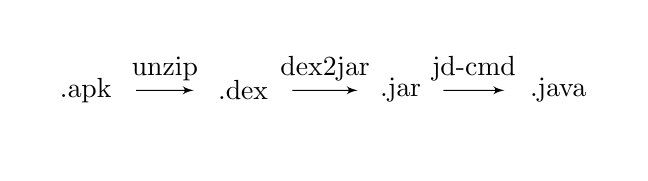
\begin{tikzpicture}[node distance = 2cm, auto]
    % Place nodes
     \node [cloud] (init) {.apk};
     \node [cloud, right of=init] (dex) {.dex};
     \node [cloud, right of=dex] (jar) {.jar};
     \node [cloud, right of=jar] (java) {.java};

     \path [line] (init) -- node {unzip}(dex);
     \path [line] (dex) -- node {dex2jar}(jar);
     \path [line] (jar) -- node {jd-cmd}(java);

\end{tikzpicture}
\caption{APK Extraction Process}
\label{fig:extractionprocess}
\end{center}
\end{figure}

\vspace{-2 mm}

\subsection{Step 3. Execute static analysis tools}
\label{sec: analysis}

The next phase was to analyze the extracted source code for a variety of metrics, including potential security risks, permissions issues, potential non-security defects, and misuse of coding standards. The tools we use  are:\\

%% Not sure this information about clones is all that relevant
%We also collected information about software clones, which are functionally equivalent portions of an application that may differ syntactically. A sign of poorly written software, clones may be detrimental to an application in a variety of ways, including increased maintenance costs and inconsistent bug fixes~\cite{Roy:2009:CEC:1530898.1531101}.

 \textbf{Stowaway:} This tool reports the overprivileges and underprivileges of an application, which we recorded. Slight modifications were made to the existing version of Stowaway to accommodate our process and current Android applications with updated permissions. %Permlyzer~\cite{6698893}, a more modern permission detection tool, was not used since its authors have not made it available for download.

 \textbf{AndroRisk} A component of the Androguard reverse engineering tool which reports the risk indicator of an application for potential malware. We recorded the reported risk level for each APK file.

AndroRisk determines the security risk level of an application by examining several criteria. The first area is the presence of permissions which are deemed to be more dangerous, such as the ability to access the internet, manipulate SMS messages, or make a payment. The second is the presence of more dangerous sets of functionality in the app including a shared library, use of cryptographic functions, and the presence of the reflection API.

 \textbf{CheckStyle:} A tool to measure how well developers adhere to coding standards such as annotation usage, size violations, and empty block checks. We recorded the total number of violations of these standards. Default settings for Android were used for our analysis.

 \textbf{Jlint:} Examines Java code to find bugs, inconsistencies, and synchronization problems by conducting a data flow analysis and building lock graphs. We recorded the total number of discovered bugs. This tool was selected over FindBugs\footnote{\url{http://findbugs.sourceforge.net/.}} since it was able to analyze the applications much faster, while still providing accurate results~\cite{rutar2004comparison}. Jlint's default settings for Android were used for our analysis.


%%% Talk about the extraction tool
% \textbf{APKParser:} A tool designed to read various information from Android APK files including the version, intents, and permissions. We used the output from this tool to determine the application version, minimum SDK, and target SDK.

\textbf{Custom APK Analysis Tool:} We built a tool to extract the requested permissions, application version, minimum SDK and target SDK from the~\emph{AndroidManifest.xml} file. We've made the tool's source code available for public use on the project website.

We also recorded other metrics about each application including total lines of code and number of Java files in the reversed engineered app.




% \todo{make sure that all these tools are relevant}


Stowaway and AndroRisk were able to analyze the raw APK files, while CheckStyle, and Jlint required the APK files to be decompiled. We also recorded the number of extracted Java files and number of lines of code (LOC). All results were recorded in an SQLite database, which is publicly available on the project website. The full analysis process is shown in Figure~\ref{fig:analysisprocess}.


\begin{figure}[h]
\begin{center}

% Define block styles
\tikzstyle{line} = [draw, -latex']

%\tikzstyle{cloud} = [draw, ellipse,fill=white!20, node distance=1.5cm, minimum height=2em]
\tikzstyle{cloud} = [draw=none, ellipse,fill=white!20, node distance=1.5cm, minimum height=2em]

\tikzstyle{block} = [rectangle, draw, fill=white!20, text width=5em, text centered, rounded corners, minimum height=4em]
\tikzstyle{c} = [draw, cylinder, shape border rotate=90, aspect=0.75, minimum height=70, minimum width=30]

\begin{tikzpicture}[node distance = 1.5cm, auto]

    % Place nodes
     \node [cloud] (init) {APK Collection};
     \node [block, below of=init] (ApkFiles) {ApkFiles};
     \node [cloud, below of=ApkFiles] (Decompile) {Decompile};
     \node [block, below of=Decompile] (DecompiledFiles) {Decompiled Files};
     \node [cloud, below of=DecompiledFiles] (JavaAnalysis) {Java Analysis};
    % \node [cloud, right of=ApkFiles] (apkanalysis) {Stowaway AndroRisk};
    % \node [c, right of=DecompiledFiles] (SqliteDB) {SqliteDB};
     \node[c] (SqliteDB) [below right=-1.0cm and 2.4cm of DecompiledFiles]{SQLiteDB};

    \node[cloud] (apkanalysis) [below right=-0.9cm and 2.0cm of ApkFiles]
       {APK Analysis};

    % Draw edges
    \path [line] (init) -- (ApkFiles);
    \path [line] (ApkFiles) -- (Decompile);
    \path [line] (Decompile) -- (DecompiledFiles);
    \path [line] (DecompiledFiles) -- (JavaAnalysis);
    \path [line] (ApkFiles) -- (apkanalysis);
    \path [line] (apkanalysis) -- (SqliteDB);
    \path [line] (JavaAnalysis) -- (SqliteDB);
    \path [line] (Decompile) -- (SqliteDB);

\end{tikzpicture}
\caption{APK Analysis Process}
\label{fig:analysisprocess}
\end{center}
\end{figure}

\section{Evaluation}
\label{sec: evaluation}


In the following sections, we describe our findings based on our analysis and answer our research questions.
%and comparisons of benign and malicious Android apps.


\subsection{RQ1: How do benign \& malicious Android apps compare in terms of quality?}
%\subsection{RQ1: How do benign \& malicious apps compare in terms of several quality metrics?\todo{reword}}

In order to better understand Android malware, we compared the static analysis results from apps collected from the Google Play store against 1,417 malware examples taken from the Contagio Mobile Mini Dump~\cite{contagio_url} and the Malware Genome Project~\cite{Zhou:2012:DAM:2310656.2310710}. The Contagio Mobile Mini Dump has been collecting malware affecting many platforms, including Android, for several years. In this study, 160 malware examples from the Contagio Mobile mini dump were used. The Malware Genome Project began in 2010 and has collected a substantial number of mobile malware. For our analysis, we used 1,257 examples from 49 malware families. %This site provided hundreds of Android malware examples, but since many of the examples in each group represented only slight alterations from one another, we selected one result from each malware family to help limit the impact that numerous results from each group would have on our overall results.

We chose to evaluate the malware samples against those collected from Google Play in a variety of areas including AndroRisk score, adherence to coding standards, discovered potential defects, over \& underprivileges, and the requested app permissions. The results of this analysis are available on our website and are summarized in Table~\ref{Table:maliciousvsnonmalicious}.

%This was accomplished by running the malicious applications through the same process as the applications collected from the Google Play store, described in Sections~\ref{sec: decompliation} and~\ref{sec: analysis}. \todo{describe what each of the sets of data mean}



\begin{table}[h]
\begin{center}
\caption{Averages for Malware vs. Non-Malicious}
\label{Table:maliciousvsnonmalicious}
  \begin{tabular}{ | l | c | c | } \hline

     \bfseries Analysis Value  & \bfseries Malicious & \bfseries Google Play \\ \hline


   % Avg. LOC /App & 30,547 & 156,515. \\ \hline   % Not sure this is a great stat to show
    Jlint Errors/LOC & 0.00298 & 0.00256 \\ \hline
    Coding Standard Mistakes/LOC & 0.055 & 0.031 \\ \hline
    Overprivileges/App & 6.2 & 3.0 \\ \hline
    Underprivileges/App & 1.9 & 3.3 \\ \hline
    Permissions/App & 12.7 & 7.7 \\ \hline
%    Opriv/Priv\dan{remove?} & 2.06 & 2.57 \\ \hline
%    Upriv/Priv\dan{remove?} & 6.86 & 2.41 \\ \hline
	AndroRisk & 56.95 & 63.28 \\ \hline

  \end{tabular}
  \end{center}
\end{table}

%%% Probably a good idea to reword all of this
%\vspace{-1 mm}
After collecting the above results we next tested the statistical significance of our findings using the one tailed Mann Whitney U (MWU) test for the hypothesis testing, since it is non-parametric and we can find out if the low-rated apps indeed have higher or lower values for each of the security metrics. The MWU test compares two population means that originate from the same population set and is used to determine if two population means are equal. A P value which is smaller than the significance level implies that the null hypothesis can be rejected. Conversely, a P value which is equal to or greater signifies that the null hypothesis cannot be rejected. In our analysis, we used a significance level of .05 to determine if we have enough data to make a decision if the null hypothesis should be rejected. As shown Table~\ref{table:studyresultsMWU}, the results of this analysis further validate our findings displayed in Table~\ref{Table:maliciousvsnonmalicious}.


%%% Mention that there is no difference between
%% \checkmark
\begin{table}[h]
\centering
\caption{MWU Results for Malicious \& Benign apps}
  \begin{tabular}{ | l | c | c | c |  } \hline
    % \bfseries Genre  & \bfseries \% of Apps \\ \hline

 & \multicolumn{2}{ c |  }{\bfseries Greater In}   \\ \hline
    \bfseries Area  &  \bfseries  Malware &  \bfseries   Google Play\\ \hline \hline

% Use \checkmark

       % Item  & X & X & X \\ \hline


    Jlint Errors/LOC  & \checkmark &    \\ \hline
    Coding Standard Mistakes/LOC  & \checkmark &    \\ \hline
    Overprivleges/App  & \checkmark &    \\ \hline
    Underpriviledges/App  &  & \checkmark   \\ \hline
    Permissions/App  & \checkmark &    \\ \hline
    AndroRisk  &  & \checkmark   \\ \hline


  \end{tabular}
\label{table:studyresultsMWU}
\end{table}





Based on our comparison of malicious apps compared to those from Google Play, we made several primary discoveries. The first is that \emph{Developers of Malware are not overly concerned with the quality of their apps:} Most Android malware is piggybacked on existing applications and malicious code is typically loosely coupled with the host application~\cite{Zhou:2012:DAM:2310656.2310710, Deshotels:2014:DAF:2556464.2556467}. We found that malicious applications had a much higher number of coding standards mistakes per LOC compared to their benign counterparts while also having a higher number of possible bugs discovered by Jlint per LOC. Although we are not able to examine the development process of malware applications or interview its developers, we are able to draw several possible conclusions. Malware developers likely care less about the actual user experience as they are not overly concerned with app quality or coding standards. This lack of attention to quality is also demonstrated by the number of overprivileges in malware compared to apps from Google Play.

Underprivileges are a quality concern since an app will likely crash if it requests a permission which it was not granted. What is somewhat surprising is that malicious apps actually have fewer underprivileges per app compared to apps from Google Play. An explanation for this could merely be that the permissions in malicious apps are more often being used, unfortunately for disruptive activities.

\emph{Malicious apps request more permissions than benign apps:} Malicious apps request an average of 12.7 permissions compared with 7.7 permissions for those collected Google Play. Malware is more likely to request these additional permissions to perform malicious activities~\cite{Sarma:2012:APP:2295136.2295141}.


We also found that \emph{AndroRisk is not a good evaluator of determining if an app is malicious:} On average, malicious apps actually had a lower AndroRisk score as compared to Google Play apps. This is a representative of the difficulties that static analysis tools have in detecting malware~\cite{4413008, Feng:2014:ASD:2635868.2635869} and should not be construed as a statement that AndroRisk is any better or worse than any other static analysis tools.



%\todo{? Talk about how this could tie into the rest of the malware detection process?}

% Much higher rate of Jlint & Coding errors in malware vs. GP
% Many more overprivs in malware, but the ratio of overpriv/app privs is actually lower. This is likely due to malicious apps making use of all requested privs for malicous reasons. This is backed up by the fact that the ratio of Overprivs/requested privs is actually lower for maliciuos apps.


% Red flags for malicious applications
% Demonstrates what malicious users like to do
% Read other papers to see what they say about permissions

%%% These values changed a bit for our most recent analysis
%%% Might not be a bad idea to run them once more



\subsection{RQ2: What are the most common permissions in Android malware?}

We next compared the requested permissions for all malicious and benign apps using a custom-built permissions extraction tool. The primary difference between requested permissions and overprivileges is that requested permissions are merely those that the app asks to use, and does not take into consideration if the app actually needs them or not.

We compared the top ten rates of requested permissions for the malicious apps against those recorded from Google Play. The results of this comparison are shown in Table~\ref{Table:permissions_usage}. The Android Malware Repository\footnote{\url{https://sites.google.com/site/androidmalrepo/permission-stats}} used a different malware oracle and found similar permissions results to what we discovered, which provides confidence to our findings. Unfortunately, they do not appear to have analyzed any apps since 2012.


%We next analyzed all 1,417 malware samples and recorded the permissions each app requested. Since the requested permissions for each app are stored in its~\emph{AndroidManifest.xml} file, we built an extraction tool to record these requested permissions. The primary difference between requested permissions and overprivileges is that requested permissions are merely those that the app asks to use, and does not take into consideration if the app actually needs them or not.



% We performed the same process on the 31,234 apps from Google Play and compared the top ten rates of requested permissions for the malicious apps against those recorded from Google Play. The results of this comparison are shown in Table~\ref{Table:permissions_usage}. The Android Malware Repository\footnote{\url{https://sites.google.com/site/androidmalrepo/permission-stats}} used a different malware oracle and found similar permissions results to what we discovered, which provides confidence to our findings. Unfortunately, they do not appear to have analyzed any apps since 2012.


\begin{table}[h]
\caption{Permissions Usage}
\label{Table:permissions_usage}
 \begin{tabular}{ | l | c | c | } \hline

  \bfseries Permission & \bfseries Malware \%& \bfseries G-Play \%\\ \hline

	INTERNET	& 98 &	94 \\ \hline
	READ\_PHONE\_STATE	& 93 &	45 \\ \hline
	ACCESS\_NETWORK\_STATE	 & 81 &	84 \\ \hline
	WRITE\_EXTERNAL\_STORAGE &	68 &	62 \\ \hline
	ACCESS\_WIFI\_STATE &	61 &	36 \\ \hline
	READ\_SMS &	60 & 	4 \\ \hline
	RECEIVE\_BOOT\_COMPLETED &	56 & 1 \\ \hline
	WRITE\_SMS &	49 &	2 \\ \hline
	SEND\_SMS &	45 &	4 \\ \hline
	RECEIVE\_SMS &	42 &	5 \\ \hline

%%% To find this I found the top privs in malware and found the correlating values for Google Play

  \end{tabular}
\end{table}

While most apps from each group request \texttt{INTERNET} and \newline \texttt{ACCESS\_NETWORK\_STATE},  we found that malicious apps requested a disproportionately high number of other permissions. 93\% of malicious apps requested~\texttt{READ\_PHONE\_STATE}, which is more than twice the average for Google Play apps. This permission is particularly dangerous since it provides the app access to a wide variety of information and functionality including verifying the user's phone with IMEI information and gathering personal information such as your phone number.

Malicious apps also requested a much higher rate of SMS related permissions including \texttt{READ\_SMS}, \texttt{WRITE\_SMS}, \texttt{SEND\_SMS} and \texttt{RECEIVE\_SMS}. Malware often propagates to other devices through SMS messages. One such example of this is~\emph{Selfmite}~\cite{zorz_zeljka_aggressive_2014}, which is an Android worm that spreads through SMS messages. SMS systems may also be abused by sending premium rate SMS messages, which could likely go unnoticed until the user receives and examines their next bill~\cite{felt2011survey}.


\texttt{RECEIVE\_BOOT\_COMPLETED} is requested 56\% of the time by malicious apps compared with only 1\% for GoogePlay apps. This permission is often used by malware to notify it that the phone has been rebooted allowing it to begin installing malicious services~\cite{canfora2013classifier}.

Malicious apps request \texttt{ACCESS\_WIFI\_STATE} 61\% of the time compared to only 36\% for apps from Google Play. This permission allows apps to access several pieces of information related to the Wi-Fi interface including accessing a user's location. Unfortunately, malicious apps have used this permission to leak personal information about the user, including their location, which they often sell to advertisers~\cite{achara2014wifileaks}.

The knowledge of what permissions have a higher prevalence in malware has several possible uses. Apps which request these permissions could be noted to have a higher probability that they are malicious. Since many benign apps have legitimate uses for these permissions, they cannot be the sole indicator, but can be an sign of a possibly malicious application. Understanding what permissions malware requests may be useful for understanding how current and future malware spreads and affects devices.

%We then examined the rates of over privileges in malicious apps compared to benign apps. The top 10 most commonly occurring over privileges, their rates, and how they differ from applications collected from the Google Play store, are shown in Table~\ref{Table:mal_permissions}.\todo{update analysis}
%\todo{keep this?}

%\begin{table}[t]
%\caption{Top Occurring Overprivileges in Malware vs. Google Play\dan{Is this useful? I think it can be meaningful data, I am just not sure how to best analyze it.}}
%\label{Table:mal_permissions}
%  %\begin{tabular}{ | p{5.3cm} | p{1.0cm} | p{1.2cm} | } \hline
 %\begin{tabular}{ | l | c | c | } \hline

  %\bfseries Permission&\bfseries Malware \%&\bfseries G-Play \% \\ \hline

%	READ\_SMS	& 60.1	& 2.8 \\ \hline
%	WRITE\_SMS	& 49 &	1.7 \\ \hline
%	CALL\_PHONE	 & 30.3 &  6.3 \\ \hline
%	WRITE\_CONTACTS	& 28.2 &	3.6 \\ \hline
%	WRITE\_APN\_SETTINGS &	25 & .5 \\ \hline
%	ACCESS\_WIFI\_STATE	& 24 &	5.9 \\ \hline
%	WAKE\_LOCK	& 20	& 2.5 \\ \hline
%	RESTART\_PACKAGES &	15.6 &	1.4 \\ \hline
%	VIBRATE	& 13.9 &	1.6 \\ \hline
%	READ\_LOGS	& 13.8 &	1 \\ \hline
%  %%% Make sure that all values are to the same decimal point

%  \end{tabular}
%%% To find this I found the top overprivs in malware and found the correlating values for Google Play
%\end{table}

%\todo{talk about how this is useful}



%%%%%%%%%%%%%%%%%%%%%%%%%%%%%%%%%%%%%%%

We next conducted a small case study on several malicious Android apps collected from the Contagio Mobile Mini Dump. The first app we selected was a fake version of Netflix, which would collect the user's information when faking a login to the Netflix service. After reverse engineering this app, we found that some of its requested privileges included \texttt{ACCESS\_NETWORK\_STATE}, \texttt{READ\_PHONE\_STATE} and \texttt{ACCESS\_WIFI\_STATE}, which are all permissions which are much more likely to be requested by malware. We selected a sample known as `LoveTrap'~\cite{LoveTrap_url1} which was originally available in a third-party app store. Some of the app's requested permissions included \texttt{READ\_PHONE\_STATE}, \newline \texttt{RECEIVE\_BOOT\_COMPLETED}, \texttt{SEND\_SMS} and \texttt{RECEIVE\_SMS} which are all much more likely to appear in malware than in benign apps. The app used \texttt{RECEIVE\_BOOT\_COMPLETED} permission to execute itself once the infected Android device was rebooted, and used the SMS related permissions to subscribe to services which may lead to unwanted charges for the infected user



% Move this to be higher up?
%% Talk about the malicious things that would specific to this app?
%   Find URLs for each of these malicious apps
% ? Do the specific privs requested match up with what I found to be malicious?

%%% DK: 8/28 - Could not find Good fake version to use

%\todo{Added this next part in}
%We next performed a case study on several specific
%
%%% Mention how these are popular
%We next compared fake, malicious copies of `Netflix' and `Player' as identified by the Malware Genome Project. A single fake copy of Netflix was included, with six fake copies of Player. We ran these fake copies of the applications against legitimate versions attained from the GooglePlay store. In both instances, the fake versions of the applications were significantly smaller than their real counterparts. We chose to only report on the Fuzzy Risk, over privilege count, and number of Java files since many of the other results of the analysis were not deemed useful due to the small size of the fake applications. The Fuzzy risk value was similar for both versions of the Netflix applications, but the real version of the Player application had a significantly higher value than its fake counterpart. The number of overprivliledges was much higher for the Fake Netflix application compared
%
%
%Full results are shown in Table~\ref{Table:fakesvsRegular}.
%
%
%
%\begin{center}
%
%\begin{table}[ht]
%\caption{Fakes vs. Regular}
%\label{Table:fakesvsRegular}
%  \begin{tabular}{ l | l | l | l }
%
%    \bfseries Application  & \bfseries Fuzzy Risk  & \bfseries Over Privileges & \bfseries Java Files \\ \hline
%    Fake Netflix & 51 & 9 & 11 \\ \hline
%    Netflix & 50 & 2 & 2429 \\ \hline \hline
%    Fake Player (Avg) & 50 & 0 & 14 \\ \hline
%    Player & 92 & 0 & 813 \\
%  \end{tabular}
%\end{table}
%\end{center}
%
%
%%% Run MWU on these?



\subsection{RQ3: Is Android Malware Growing?}

We next compared how Android malware has grown over the years in comparison to benign apps collected from Google Play. We separated the apps collected from the Contagio Mobile Mini Dump into those created in or before 2012, 2013, 2014, and 2015. We did not use apps from the Malware Genome Project since we were unable to collect accurate date information for these apps. The results of this analysis are shown in Figure~\ref{fig:malwareEvolutionLOC}.

 %while Figure~\ref{fig:malwareEvolutionPrivs} shows the growth in both the overprivileges, and permissions requested by malware.\todo{? Talk about the number of apps analyzed}


%%% Number of apps analyzed
% 2011		1
% 2012		8
%	<=2012	9
% 2013		69
% 2014		51
% 2015		28



% Describe the data a bit more and what it means?


%% Mention the number of apps collected from each group to further demonstrate that these numbers are accurate
%% Double check the results


%\begin{table}[h]
%\centering
%\caption{Evolution of Contagio Malware \dan{put data into different format? I am not sure what the best format would be}\todo{make sure this data adds up to other collected results}}
%\label{Table:malwareEvolution}
%\begin{tabular}{ | l | c | c | c | c | c | } \hline
%
% \bfseries Year & \bfseries JavaFiles			 & \bfseries OverPrivileges & \bfseries Privilege Count \\ \hline
%
%%	$\leq $ 2012 & 	223.33 &	54 & 	0.22 & 	0.02 & 	1.78 &	7.78 \\ \hline
%%	2012 & 	X &		X & 	X &	 X  \\ \hline
%%	2013 & 	330.65 &		2.34 & 	3.6 &	 10.21 \\ \hline
%%	2014 &  726.66 &		2.05 & 	4.54 &	12.43 \\ \hline
%%	2015 & 	774.56 &	3.34 &		6.61 &	17.39 \\ \hline
%
%	$\leq $ 2012 & 	223 &	1.98 &	 7.8  \\ \hline
%%	2012 & 	X &		X & 	X &	 X  \\ \hline
%	2013 & 	331 & 4.7 &	 10.7  \\ \hline
%	2014 & 	 618 & 7.8 &	 13  \\ \hline
%	2015 & 	1263 & 8 &	 18.2  \\ \hline
%
%  \end{tabular}
%\end{table}



\definecolor{bblue}{HTML}{4F81BD}
%\definecolor{rred}{HTML}{C0504D}
\definecolor{ggreen}{HTML}{9BBB59}
%\definecolor{ggrey}{HTML}{707070}

%%%% -----------
%% Colors used for bar chart


% 100000

\begin{figure}[h]
%\vspace{-0.05in}
\begin{tikzpicture}
\begin{axis}[
    ybar,
%	scale only axis,
    enlargelimits=0.15,
    legend style={at={(0.5,.9)},
      anchor=north,legend columns=-1},
      ylabel=LOC (100K),
%   ylabel={\#participants},
    symbolic x coords={$\leq $ 2012,2013,2014,2015},
    xtick=data,
%    nodes near coords,
%    nodes near coords align={vertical},
	xticklabel style={text width=4em, font=\small},
	bar width=12pt
    ]


%%%% This was for Java Files
%%% Malware
%\addplot [style={ggreen,pattern=north east lines,mark=none}]coordinates {($\leq $ 2012,223)(2013,331)(2014,618)(2015,1263) };
%
%%% GP
%\addplot [style={bblue,pattern=dots,mark=none}]coordinates {($\leq $ 2012,336)(2013,784)(2014,1650)(2015,2141) };



%%% For LOC
%% Malware
\addplot [style={ggreen,pattern=north east lines,mark=none}]coordinates {($\leq $ 2012,17693.375)(2013,32988.662)(2014,74606.432)(2015,109947.075) };

%% GP
\addplot [style={bblue,pattern=dots,mark=none}]coordinates {($\leq $ 2012,35645)(2013,86482)(2014,181225)(2015,229355) };




\legend{Malware, Benign}
\end{axis}
\end{tikzpicture}
\caption{Evolution of Malware Size in LOC}
\label{fig:malwareEvolutionLOC}
\end{figure}


%\begin{figure}
%%\vspace{-0.05in}
%\begin{tikzpicture}
%\begin{axis}[
%    ybar,
%% scale only axis,
%    enlargelimits=0.15,
%    legend style={at={(0.5,1.2)},   % orig:    legend style={at={(0.5,-0.25)},
%      anchor=north,legend columns=-1},
%%   ylabel={\#participants},
%    symbolic x coords={$\leq $ 2012,2013,2014,2015},
%    xtick=data,
%%    nodes near coords,
%%    nodes near coords align={vertical},
%  xticklabel style={text width=4em, font=\small},
%  bar width=12pt
%    ]
%
%%% GP Apps
%%2011 = 2.3 - 3.9
%%2012 =2.3 - 5.1
%%2013 =2.6 - 6.3
%%2014 =3.1 - 8.2
%%2015 = 3.4 - 8.8
%
%% Use a grouped bar chart?
%% http://tex.stackexchange.com/questions/101320/grouped-bar-chart
%
%%% OverPrivs - GP
%%\addplot [style={bblue,pattern=dots,mark=none}]coordinates {($\leq $ 2012,2.3)(2013,2.3)(2014,2.6)(2015,3.1) };
%
%
%%% OverPrivs - Malware
%\addplot [style={ggreen,pattern=north east lines,mark=none}]coordinates {($\leq $ 2012,1.98)(2013,4.7)(2014,7.8)(2015,8) };
%
%
%
%%% Permissions - Malware
%\addplot [style={bblue,pattern=dots,mark=none}]coordinates {($\leq $ 2012,7.8)(2013,10.7)(2014,13)(2015,18.2) };
%
%
%
%
%\legend{Overprivileges, Permissions}
%\end{axis}
%\end{tikzpicture}
%\caption{Malware Overprivileges \& Permission Count\todo{Add in regular app privs? Might overcomplicate things?}}
%\label{fig:malwareEvolutionPrivs}
%\end{figure}


This data indicates that both malware and benign apps are growing in terms of LOC on a yearly basis, although benign apps are typically larger. %\todo{add more1}





%This data provides us several key findings:
%\emph{Malware is getting larger \& is requesting more permissions:} In $\leq $ 2012 , malware had an average size of 223 Java files, while in 2015 they grew to have an average of 1263 Java files per app. A possible explanation for this is that malware is making use of more third party libraries, or is making more of an attempt to masquerade as legitimate apps. While we found that benign Android apps are also growing, we found that malware is growing at a disproportionably high rate. Malicious apps have also been steadily requesting a larger number of permissions going from an average of 7.8 in malware created $\leq $ 2012  up to 18.2 apps in 2015. Although Google has been releasing an increasing number of permissions in each API release of Android, the growth rate of permissions requested by Android apps far exceeds the rate that Google is releasing new permissions. The rate of overprivileges is also increasing from only 1.98 in $\leq $ 2012 to 8 in 2015. This indicates that malware developers are not only requesting more permissions that are being used, but permissions which are not being used.

%% Is there another year (2012) that can be added to this equation.
%% How about comparing it to GooglePlay info? Show if both groups are evolving at the same rate


%We next looked to see how these results compared with trends from apps from Google Play. We compared the number of Java Files and requested permissions for apps $\leq $ 2012 , 2013, 2014, 2015. These results are shown in Figure~\ref{fig:GP_Mal_Evolution}. In order to assist in the data representation, the number of Java files has been divided by 10 in this chart.

%\begin{figure*}
%\begin{center}
%\begin{tikzpicture}
%\begin{axis}[
%   smooth,
%   width=18cm,
%   height=6cm,
%   enlargelimits=0.15,
%	xlabel={Year},
% %  ylabel={Values},
%  symbolic x coords={$\leq $ 2012 , 2013, 2014},
% xtick=data,
%  x tick label style={rotate=0,anchor=north},
 % legend pos=north west, font=\small, ,line width=.8pt,mark size=.2pt,
% axis y discontinuity=parallel,
%  ]	


%\addplot+[color=blue,densely dotted,mark=*,mark options={solid},smooth] plot coordinates {($\leq $ 2012 ,2.2) (2013,3.35) (2014,6.18) };
%\addlegendentry{Java Files - Malware}

%\addplot [color=red,loosely dotted,mark=*,mark options={solid},smooth] plot coordinates {($\leq $ 2012 ,2.21) (2013,3.79) (2014,7.84) };
%\addlegendentry{Java Files - Google Play}


%\addplot+[color=orange,solid,mark=*,mark options={solid},smooth] plot coordinates {($\leq $ 2012 ,7.78) (2013,10.49) (2014,12.98) };
%\addlegendentry{PrivCount - Malware}

%%\addplot [color=green,solid,mark=*,mark options={solid},smooth] plot coordinates {($\leq $ 2012 ,3.9) (2013,5.1) (2014,6.4) };
%%\addlegendentry{PrivCount - Google Play}

%%\addplot [color=blue,dashed,mark=*,mark options={solid},smooth] plot coordinates {(0,3.5) (1,2.17) (2,2.55) (3,3.14) (4,3.43) (5,4.5)};
%%\addlegendentry{Music \& Audio}

%% In this case, there were no resulst returned for puzzle for overprivs
%\addplot [color=black,dashdotted,mark=*,mark options={solid},smooth] plot coordinates{(0,1) (1,1.93) (2,2.1) (3,3.92) (4,1) (5,2.33)};
%%\addlegendentry{Puzzle}

%%\addplot [color=green,solid,mark=*,mark options={solid},smooth] plot coordinates {(0,1.5) (1,1.96) (2,2.56) (3,2.12) (4,2.41) (5,2.89)};
%\addlegendentry{Education}



%\end{axis}
%\end{tikzpicture}

%\caption{Evolution of Google Play vs. Malware\dan{remove this?. I am not sure how much value add it has}\todo{Add in 2015?}}
%\label{fig:GP_Mal_Evolution}
%\end{center}
%\end{figure*}

%This demonstrates that malware is growing both in number of requested permissions and overall size in relation to its benign counterpart from Google Play. However, malicious apps continue to request a significantly higher of permissions.

%%% Compare these permissions to those requested in GP apps



% Next compare each permission and what happens to them over the years
%We next broke each requested malicious privilege into three groups, those from malware created in 2013 and those years previous, 2014, and 2015. We then chose five permissions that became





%\todo{Add more findings}




%% Examine a few apps from each group






%\dan{Do an analysis on a specific malicious app and compare that to a "regular" one? }


%We will next perform a case study on a specific malicious app. For this analysis, we selected................



%% Look at how requested permissions have been evolving






%%%%% Studies of specific apps

%\textbf{Rogue Lemon}
%- Available in chinese markets
%-


% F-Risk: 50
% Jlint: 164
% Defect: 3
% OPriv: 5
% Privs : 14



%%%

%   How was the app created.
%   What is the vulnerability. What damage did it cause?
%   What did we find in our analysis
%       What do the oprivs do
%       How do the apps permissions tie into our list of permissions?

%   Analyze the app


%%% - Probably have one table with all app info
% F-Risk: X
% Jlint: X
% Defect: X
% OPriv: X
% Privs : X


%http://www.csc.ncsu.edu/faculty/jiang/RogueLemon/





%6 -http://www.csc.ncsu.edu/faculty/jiang/RogueLemon/


%AnserverBot10 - http://www.csc.ncsu.edu/faculty/jiang/AnserverBot/


%zhash 18 - https://blog.lookout.com/blog/2011/03/20/security-alert-zhash-a-binary-that-can-root-android-phones-found-in-chinese-app-markets-and-android-market/







%   Find apps
%       That have supporting websites
%       That represent different things that we are trying to show.


%	Apps developed quickly. Very poor quality
%	Apps with just too many permissions


%




%%%%%%%% Not sure what to do about this







%The~\emph{WRITE\_EXTERNAL\_STORAGE} was the most occurring over permission an malicious applications. This permission is used to store information on an external storage device such as an SD card and is often used by malicious applications

%- Many of the other requested permissions are not surprising since they may be used to gather

% Analyze these---- Can over permissions be used by malware





\section{Public Dataset}
\label{sec:dataset}


Our project website is located at \textbf{\ifisnopii \url{http://darwin.rit.edu/amp/} \else http://hiddenToKeepAnonymous\fi} and we have made our data set available for future researchers to use in their own studies. The raw data used in our analysis is available in three SQLite databases, with one each for the malware data from Contagio and the Malware Genome projects, and a third for the collected information from Google Play.

The databases schemas are constructed in a similar format to one another and contain views that make data analysis easier. Further information regarding these views, along with ER diagrams to visually represent the dataset are available on the project website. The website also contains prebuilt reports with data available in a variety of formats including html, pdf, xls, and csv; users are also able to build their own reports. Unfortunately, the actual malicious APK files may only be obtained from the Contagio and Genome websites due to usage agreements.

%A screenshot of an example report showing the top occurring overprivileges in malware from 2014 is shown in Figure~\ref{fig:fakewebsitereport}.


%%%%% Use an image to demonstrate the data exists
%\begin{figure}[ht!]
%\centering
%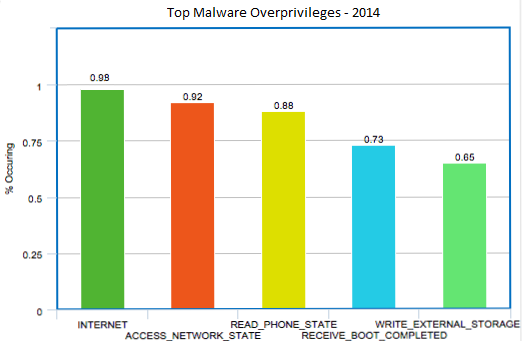
\includegraphics[width=0.49\textwidth]{images/fake_malware_barchart.png}
%\caption{Example Overpriviledge Report from Website}
%\label{fig:fakewebsitereport}
%\end{figure}

%% Talk about how this






% Clearly explain where others can find our data
% Describe how others can use the results


% The SQLite Data is available on our project page
%	Clearly describe which data is which
%	Provide an ER diagram for the data
% 3 SQLite databases
%	GP
%	Contagio
%	Genome Project
% Bult in views to assist with reports and analysis
% Data will be updated as new malware and benign apps are collected

% Describe how aggregate malware information can be used



%While the actual malicious apps may only be attained from the Contagio and Genome websites due to usage agreements, we will be providing a SQLite database containing our results on our project website located at: \textbf{\ifisnopii \url{http://darwin.rit.edu/amp/} \else http://hiddenToKeepAnonymous\fi}. In addition to the raw data which may be used by future researchers, the database also contains several views which should make future analysis easier. Further information regarding these views, along with ER diagrams to visually represent the dataset are available on the project website.

%%% Reports are available in several formats. HTML, .csv, pdf, xls, raw SQLite

%There are innumerable uses for this dataset by future researchers. Researchers of malicious Android apps could use \todo{finish}


%Extend upon our work



% \dan{? What would be a good sample set of data to show here?}



\section{Limitations \& Future Work}
\label{sec:limitations}

While we have achieved interesting and profound results, our work is not without its limitations. We relied upon several static analysis tools for our results. While these tools have been substantially used in previous research, no static analysis tool is perfect and generally inherently contain limitations~\cite{chess2004static}. However, we believe that our results based on these static analysis tools are accurate, since other works have found them to produce accurate results~\cite{apvrille2012android,chawla2014transfiguring}, and also due to the magnitude of the apps in our study.


We measured the adherence to coding standards using CheckStyle, a popular static analysis tool. We only evaluated apps against the default Android settings for this tool, which could create issues since groups rely upon a variety of different coding standards. This means that an app could perfectly adhere to a company's specific coding standards, but still have violations reported by the tool. While this will lead to inaccuracies using any single coding standard benchmark against a variety of apps, we feel that this issue does not significantly impact our results since we used the same benchmark for such a large number of apps at an aggregate level and thus our basic findings will be unchanged. When using Jlint, we may only assume that \emph{potential} defects are found. Actual defects should only be identified through manual analysis, and no single static analysis tool should ever be solely relied upon to discover actual defects.


While we can reasonably assume that the vast majority of apps from Google Play are benign, it is likely that several malicious applications have successfully circumvented Google's protection mechanisms. However, even if this is the case, we believe that it would be a statistically insignificant portion of the apps.

Although we analyzed a substantial number of benign and malicious apps, we obviously only examined a very minor portion of all apps. We believe that our results accurately represent each group and that it is unreasonable to expect and study to examine all possible apps.

A large portion of malware is piggybacked on legitimate apps, so many of our results may be skewed by the fact that an overwhelming portion of a malicious app may have originally been legitimate. The significant differences discovered between malicious and benign apps help to alleviate this concern.
%Finally, malware is constantly evolving and our discoveries with current malware do not necessarily mean than future malware will have the same tendencies.


% Stats obviously vary on the precise apps which are analyzed. For exmaple, we found that XXX\% of apps requested \texttt{ACCESS\_WIFI\_STATE}, while a recent study found that 41\% of apps from Google Play requested this permission~\cite{achara2014wifileaks}. We feel that the XXX\todo{update} apps we collected are a good representation of Android apps and that no analysis can every be considered to be completely precise unless it were to evaluate all Android apps, which is not practical.


%\section{Future Work}
%\label{sec:futurework}


We have presented novel results, but there is still room for building on our work. A natural next step is to study more malicious and benign apps. Apps could also be broken down into groups, such as genres. Malware could also be examined at different levels of granularity. The primary purpose of our study was to understand malware at a higher, more aggregate level, but there is always a need to perform lower, more in depth studies to examine malware at a much more granular level. One example could be to study how malware uses various Android libraries and other components. Finally, our study could largely be applied to various other types of software including iOS apps.

We chose to use the Mann Whitney U analysis to add confidence in our comparison of malicious and benign apps. However other correlation metrics such as the Spearman, Kendall, or Pearson rank correlations may also be used in future research.

%%% Right from the user ratings paper.
%We chose to use the Mann Whitney U analysis of high-rated vs. low-rated apps, however other correlation metrics such as the Spearman, Kendall or Pearson rank correlations may also be used. The Spearman rank correlation coefficient is also a non-parametric, and measures the strength of association between two ranked variables. Kendall's evaluates the strength of dependence between two variables. Pearson r is often used to measure how much two items are related to one another. We are confident in our decision to use the MWU analysis in our study, due to its ability to state if the median values of two sets of data are significantly different from one another. However, future work cold be done to use the Spearman, Kendall or Pearson correlation metrics as well.


%An additional study could take place to examine the permissions


% A more long term study on Android malware
% Did not break premissions down based on severity (normal, dangerous etc..)



%\pagebreak
\section{Conclusion}
\label{sec: conclusion}
In order to better understand Android malware, we compared 1,417 malicious apps against 31,234 benign apps collected from Google Play using a variety of static analysis tools. Our primary findings were that malware developers typically pay far less attention to app quality as compared to benign apps. Several permissions, specifically SMS related privileges, are much more common in malware, and that malware is growing both in terms of app size and requested permissions. We have also made our data set public for future researchers.




% Briefly Highlight some of our major findings
%


% \textbf{\ifisnopii \url{http://darwin.rit.edu/amp/} \else http://xxx.hidden.xxx \fi}

\section*{Acknowledgements}

\ifisnopii % turn on/off pii
\todo{put information in here}
\else % turn on/off pii
Author and funding acknowledgments hidden for review anonymity.
\fi % end turn on/off pii


\balance
\bibliographystyle{abbrv}
\bibliography{AndroidData}



% That's all folks!
\end{document}

%%%% ************ Final Submission info for SAC 2016 *****************

% Confirmation Number:	1103
% Submission Passcode:	1103X-J5P3A2A3H9
%   https://www.softconf.com/f/sac2016/cgi-bin/scmd.cgi?scmd=aLogin&passcode=1103X-J5P3A2A3H9

% Make sure it is clearly labeled to be potential defects from Jlint and other static analysis tools




%%%% *****************************





%   Due date: September 11, 2015 - http://selab.uos.ac.kr/sacse16/
%   Queries located at: https://docs.google.com/document/d/1-z0AsZFgbz8UF2j0eLyw5Tp7YhJFczjARBgrwebqURw/edit
%   	Make sure keywords and formatting is all set
%   	Use the term "overprivilege"
%   Make sure "Blind" version of paper hides all identifiable info and proofread with that info


% &&&&&&&&&&&&&&&&&

%   What comments were made about the SAC papers that did not get in last year?
%   Add in a small section for Recommendations - How could these problems be solved by developers
%   Make sure it is "AndroRisk" - case sensitive



%%%%% Other RQs
%	Do developers make use of new Android permissions?
%	Do people use new API versions?
%   Would need to hook this into dates as well. Demonstrate that apps were able to swtich APIs
%	Could we argue that using these metrics could be a red flag for detecting malware
%	? Break down permissions by number of dangerous ones




% Interesting paper - PlayDrone
%   http://engineering.columbia.edu/columbia-engineering-team-finds-thousands-secret-keys-android-apps-0
%   Make sure that all the numbers (rates especially) in the charts & tables add up appropriately
% DREBIN: Effective and Explainable Detection of Android Malware in Your Pocket


%	Create website to accompany findings
%		Both regular website and GH pages.
%		Top permissions
%		Permissions in each each
%		<<Basically look at excel tab>>



% Todo
%   Dataset or Data Set
%   Use the term "overprivilege"
%   Really work on refining the datat we have. What analysis can we do? Interesting findings?



